\section{Introduction}
\label{sec:intro}
% \MY{Title: The more the merrier: mixed Chain-of-Psychotehrapy-Thoughts for mental health support}
Mental health plays a crucial role in personal well-being, yet there's a shortage of specialized mental healthcare resources worldwide~\cite{Sharma_Choudhury_Althoff_Sharma_2020}. To bridge this gap, AI-driven chatbots have emerged as promising solutions~\cite{welivita-pu-2023-boosting}. These chatbots function as virtual counselors, offering convenient avenues for individuals to access support in their daily lives. 
% Within these interactions, empathy plays a pivotal role, fostering engagement and prompting help seekers to share more openly, thereby facilitating tailored support~\cite{lahnala-etal-2022-critical}.


\begin{figure}[th]
	\centering
	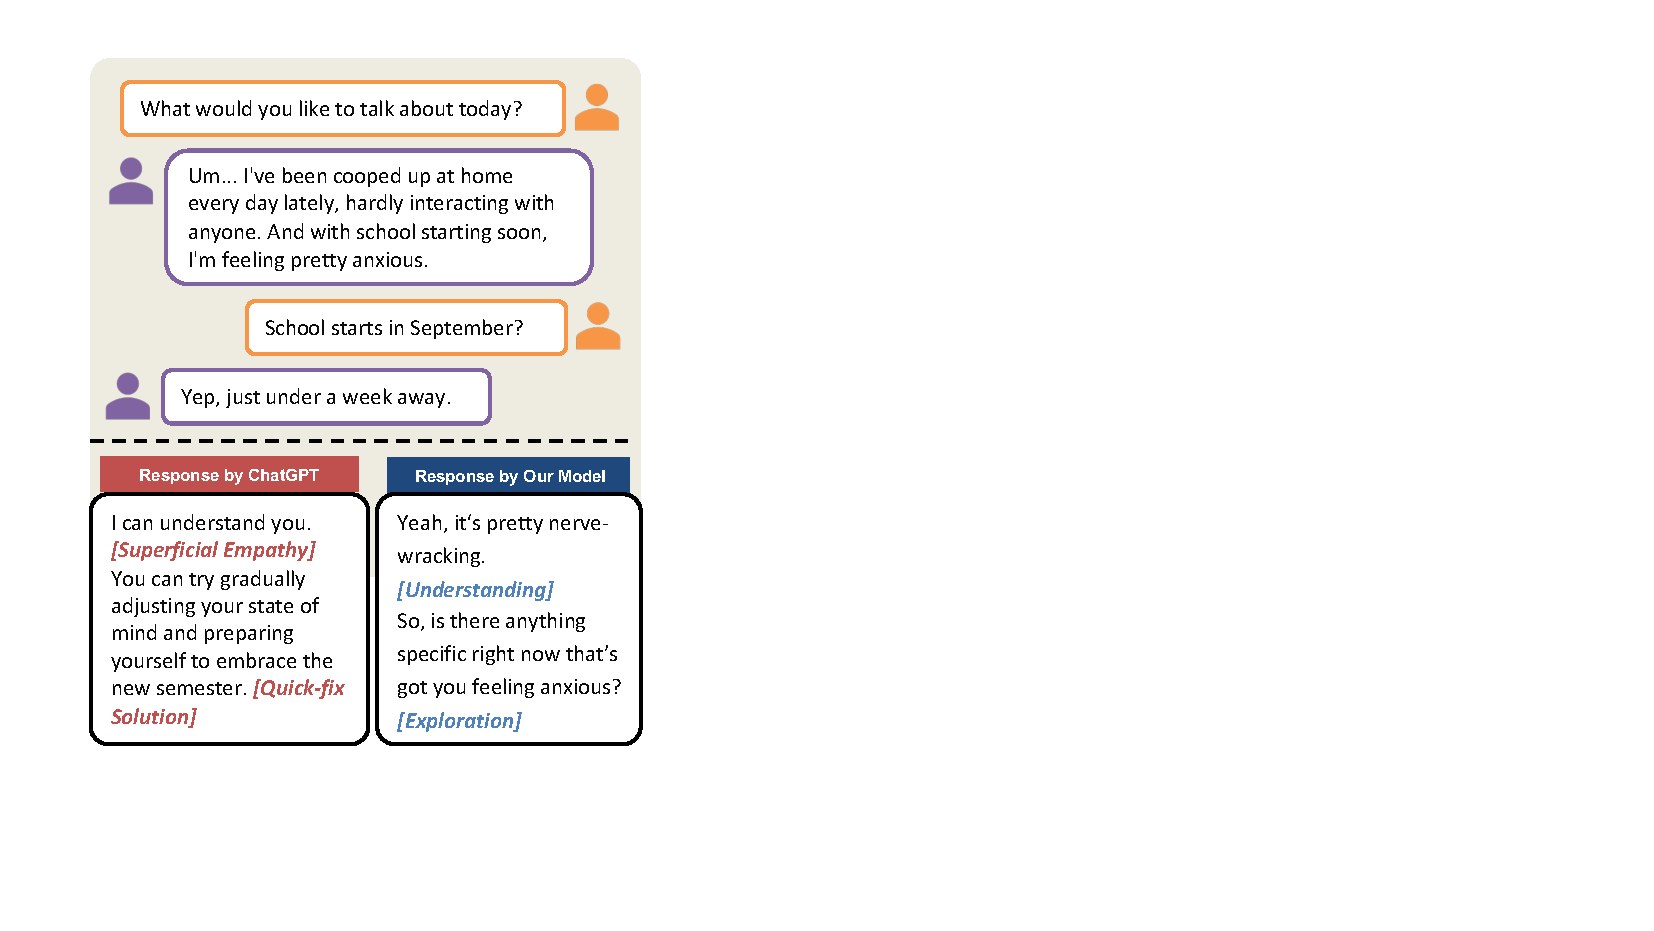
\includegraphics[width=0.8\linewidth]{figures/overview.pdf}
	\caption{Comparison of the responses generated by ChatGPT and \textit{PsyMix} based on the same context.}
 % \KZ{Shouldn't SFBT CoT, CBT CoT and PCT Cot point to SFT LLM instead of the reponse?}}
	\label{fig:overview}
\end{figure}

Numerous attempts have been made to develop mental health support chatbots, particularly in the era of Large Language Models (LLMs). However, current approaches~\cite{Qiu2023SMILEST, loh2023harnessing, Chen2023LLMempoweredCF} simulating counselors by prompting LLMs fall short on several dimensions compared with real-life counselling sessions.
The first one can be termed as ``\textit{\textbf{superficial empathy}}'', which manifests as vague and generalized responses aimed at conveying empathy (e.g., ``I can understand your feelings''). These responses lack profound and specific comprehension of the user's context, potentially leaving them feeling inadequately understood~\cite{lee-etal-2023-empathy, Sharma2021Empathy}.
Another issue is referred to as ``\textit{\textbf{Quick-fix Solution}}'', as LLMs tend to offer general solutions as soon as the user expresses concerns, without exploring the underlying reasons or less apparent issues. These quick fixes are usually insufficient to align with the nuanced requirements of mental health support~\cite{Sharma_Choudhury_Althoff_Sharma_2020}, where counselors should encourage self-exploration to provide tailored support~\cite{lahnala-etal-2022-critical}.

Both of these issues stem from a lack of comprehensive understanding and professional insight into seeker's situation through the application of psychotherapy knowledge. 
Drawing inspiration from real counseling scenarios, where seasoned counselors often blend various psychotherapy approaches to analyze the seeker's situation~\cite{lee2023chain}, we endeavor to integrate multiple mainstream therapy approaches into LLM tuning for mental health support. 
However, modeling after human counselors poses several challenges: 1) the internal analysis performed by a counselor is not explicitly conveyed in their responses, making it difficult to replicate this cognitive process; 2) there currently lacks datasets that differentiate counseling dialogues by psychotherapy approach. Moreover, since counselors often blend approaches, distinguishing between them may also be inherently unnatural. Consequently, there is an absence of dialog datasets with psychotherapy-related annotations.

% \MY{Not just understanding, but using psychotherapy knowledge/theory to understand}. 
% \MY{You can also say here that in real sessions, counsellors usually involve more than one therapy types. Inspired by this mixture of thinking in counselling sessions, we propose Mixed CoT that integrates a plethora of mainstream therapy types in mental health support LLM tuning.}
% Our solution draws inspiration from real counseling scenarios, where counselors typically select the appropriate psychotherapy approach to analyze the seeker's situation before providing responses~\cite{}. Moreover, experienced counselors often employ a combination of various psychotherapy approaches during interactions with seekers~\cite{lee2023chain}. 

Therefore, our work seeks to overcome these hurdles by introducing \textit{PsyMix}, a conversational agent designed for mental health support. To tackle the intricacy of integrating expert knowledge, we leverage ChatGPT to reconstruct the analysis of seekers' situations at the sentence level. 
With expert-directed dimensional guidelines, we generate professional analyses from the viewpoints of various psychotherapy approaches (such as cognitive behavioral therapy, CBT) for each response in existing pure-dialog datasets provided by human counselors~\cite{li-etal-2023-understanding}, and these analyses are denoted as \textbf{\textit{Chain-of-Psychotherapies (CoP)}}. 
Subsequently, we employ supervised fine-tuning (SFT) to tune an LLM using data featuring mixed analyses from diverse psychotherapies. These analyses guide the response generation process, enhancing the agent's ability to deliver tailored support. Experimental results demonstrate the superiority of our approach with CoP over naive SFT methods. Additionally, the integration of mixed CoP in the tuning data enables insights from diverse analytical perspectives, further improving performance over single-aspect CoP methods.

% single-aspect CoT baselines, exhibiting a level of empathy in responses comparable to that of human counselors. 



% \MY{consider rewrite the last sentence: with CoP results are improved, further elevated by PsyMix}

% \KZ{I find it hard to believe that other previous work was not inspired by real experienced therapists and didn't try to model after them. The challenge is perhaps HOW to model after these experts.} 


% \MY{Intro part is a bit messy now, your challenges are scattered, try grouping them together logically: current bots are not good enough (this is clear), and we can use therapy theories to help, while simulating these theories is difficult because of xxx (reasons are listed clearly in your original text). Therefore, we propose xxx. This method has xxx benefits and our results show xxx. (The only weakness now is that we say that simulating is difficult, but the method being proposed is CoT, which is a common solution. I still think we should focus on mixture part)}

% Our main contributions in this paper are as follows:
% \begin{itemize}
%     \item We introduce PsyMix, a mental health support chatbot focus on enhancing empathy through a mixture of analysis from multiple psychotherapy approaches. \KZ{Are we the first to do that, if so, say it.}
%     \item We extensively evaluate chatbots using GPT-4 and human evaluations. Our method demonstrates significant improvements over naive supervised fine-tuning in various aspects.
% \end{itemize}
% By emulating this flexibility in analyzing seekers' situations with multiple psychotherapy approaches, our chatbot can better understand seekers' situation and provide more empathetic responses.
% Our objective is to enhance empathy through a better understanding of the seeker's situation, reducing authoritarian quick-fix solutions.

% Empathy holds significant importance in conversations, particularly in scenarios involving emotional support~\cite{liu-etal-2021-towards} and psychological counseling~\cite{li-etal-2023-understanding}. 
% Numerous efforts have been made to incorporate empathy into chatbots. 
% Some approaches~\cite{Saha2022Motivational,zheng-etal-2023-augesc} focus on implementing counseling strategies, such as Hill's Helping skill~\cite{Hill2009Helping} or strategies from Motivational Interviewing~\cite{Miller1995MI}, to make responses appear more empathetic. However, these strategies often fall short in fully grasping the client's situation, leading to ``superficial empathy'' (refer to Figure \ref{fig:overview} for example). This phenomenon has been highlighted in previous study~\cite{lee-etal-2023-empathy, Sharma2021Empathy}. Merely using patterned statements like ``I can understand your feelings'', regardless of context, can result in high scores in current empathy benchmarks~\cite{sharma-etal-2020-computational}, which is not reflective of genuine empathy.

% First, there's a deficiency in modeling from the seeker's perspective. Many existing solutions~\cite{Saha2022Motivational,zheng-etal-2023-augesc} tend to focus on implementing counseling strategies to enhance empathy. However, this often results in ``superficial empathy'', characterized by vague and generalized responses. For instance, phrases like ``I can understand your feelings'', lack a deep understanding of the seeker's situation, potentially leaving them feeling inadequately understood~\cite{lee-etal-2023-empathy, Sharma2021Empathy}.
% Secondly, recent attempts~\cite{Qiu2023SMILEST, loh2023harnessing, Chen2023LLMempoweredCF} at simulating counselors or psychiatrists by prompting LLMs tend to lean towards providing quick-fix solutions, which can result in offering general remedies without fully understanding the seeker's situation. Additionally, these chatbots may occasionally adopt an authoritarian tone. Such traits may not always align with the nuanced requirements of mental health support scenarios, in which the counselor should encourage the help seeker to express themselves~\cite{Sharma_Choudhury_Althoff_Sharma_2020}. 

% The second issue often occurs in recent works which simulating counselors or psychiatrists by prompting LLMs~\cite{Qiu2023SMILEST, loh2023harnessing, Chen2023LLMempoweredCF}. These chatbots, solely driven by prompts, tend to offer perfunctory solutions and occasionally adopt an authoritarian attitude~\cite{zhou2023think} (See Figure \ref{fig:overview} for example). Such traits may not always align with the nuanced requirements of mental health support scenarios, in which the counselor should encourage the help seeker to express themselves~\cite{Sharma_Choudhury_Althoff_Sharma_2020}. 
% resulting in . This is characterized by vague and generalized responses that lack a deep understanding understanding of seeker's situation, such as ``I can understand you''~\cite{lee-etal-2023-empathy, Sharma2021Empathy}. 
% many~\cite{Saha2022Motivational,zheng-etal-2023-augesc} tend to focus on implementing counseling strategies, 
% such as Hill's Helping skills~\cite{Hill2009Helping}, 
% viewing the issue from the counselor's perspective. However, these approaches often lack depth in understanding the client's situation, resulting in ``superficial empathy'', characterized by vague and generalized responses, such as ``I can understand you''~\cite{lee-etal-2023-empathy, Sharma2021Empathy}. 
% This phenomenon has been highlighted in previous study. 
% For example, merely using patterned statements like ``I can understand your feelings'', regardless of context, can  inflate scores on current empathy benchmarks~\cite{sharma-etal-2020-computational}, failing to reflect genuine empathy. 
% To tackle this challenge, some previous studies have shifted focus to the seeker's perspective by categorizing the seeker's emotions~\cite{rashkin-etal-2019-towards} or behaviors~\cite{qiu2023psychat} before generating responses. However, such categorization is constrained by the taxonomy employed, limiting scalability.


% In the era of Large Language Models (LLMs), the scalability challenge can be effectively solved by leveraging LLMs, which are equipped with abundant knowledge. Recent studies~\cite{Qiu2023SMILEST, loh2023harnessing, Chen2023LLMempoweredCF} have utilized LLMs like ChatGPT to simulate counselors or psychiatrists, often employing techniques such as the Chain of Thought (CoT) prompting~\cite{Wei2022CoT} to enhance the analysis of client situations.
% However, these chatbots, simply driven by prompts, tend to offer quick solution \KZ{What do you mean by quick solution, and why is it necessarily bad? Did you mean ``quick fix'', or ``perfunctory fix''} and occasionally adopt an expert-like \KZ{Why is expert necessarily bad? Maybe you wanna say authoritarian?} attitude~\cite{zhou2023think} (See Figure \ref{fig:overview} for example). Such traits may not always align with the nuanced requirements of mental health support scenarios, in which the counselor should encourage the help seeker to express themselves~\cite{Sharma_Choudhury_Althoff_Sharma_2020}. 

% In contrast, utilizing real mental health support dialogue data to fine-tune LLMs can better enable chatbots to learn the language style and counseling methods of therapists, providing a more engaging conversational experience.

% Secondly, since LLMs are primarily designed as assistants to provide effective solutions to users' problems, they often offer multiple general solutions as soon as the user expresses concerns, without exploring the underlying reasons or less apparent issues. This quick fix is not align with the nuanced requirements of mental health support scenarios~\cite{Sharma_Choudhury_Althoff_Sharma_2020}, where counselors should encourage the help-seeker to delve deeper into self-exploration, thereby facilitating tailored support~\cite{lahnala-etal-2022-critical}.
